\section{Результаты}
\begin{frame}
	
	\frametitle[	содержимое...]{Результаты в цифрах}
	\begin{itemize}
		\item<+-> Пройдено \textbf{111} км за \textbf{13} ходовых дней
		\item<+-> Получился такой высотный график:
		\item<+-> Граммовка раскладки~--- в среднем \textbf{500} граммов на человека в день
		\item<+-> Продолбано \textbf{6} участников из 12
		\item<+->Средний расход аптечки:
	\end{itemize}
	
	\only<2>{
		\begin{center}
			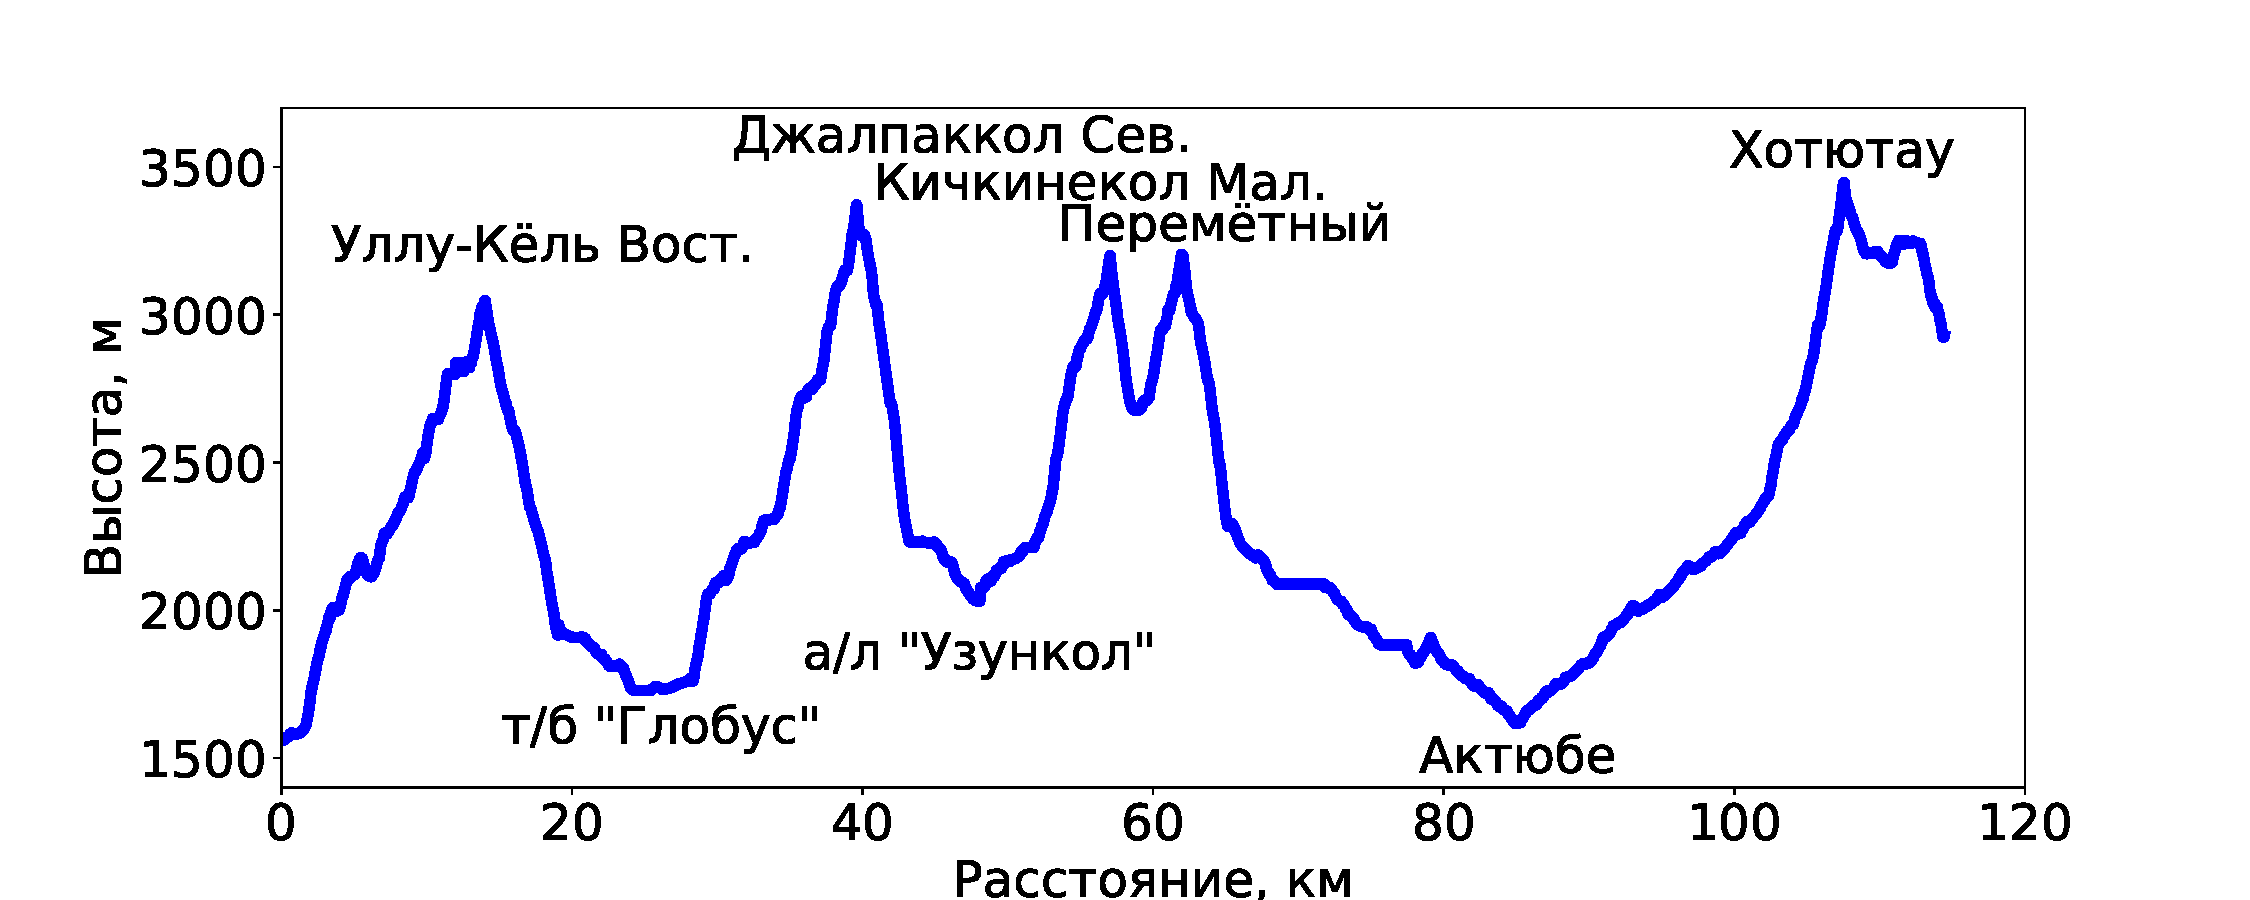
\includegraphics[width=\textwidth]{../pics/elevation_vs_distance}
		\end{center}
		\vfil
	}
\end{frame}

